%\chapter{Bayesian Neural Networks for Cancer Types Prediction}
%\chapter{Neuro-symbolic Representation Learning on Knowledge Graphs}
\chapter{Explaining with Decision Rules}\label{chapter:xai_rules}
\textit{``Compass rules direction; Decision rules life! ''}- Israelmore Ayivor

\section{Chapter Overview} \label{chapter_7:cw}
With the growing adoption of machine learning~(ML), there is a surge of research interest towards making ML models more transparent and interpretable~\cite{ming2018rulematrix}. In the previous chapters, we provided visualization plots to  explain clinical decisions. Those were mostly suitable for an ML expert, e.g., data scientist. However, a large number of potential but neglected users are the domain experts with little knowledge of ML but are expected to use such an XAI system in a clinical setting~\cite{ming2018rulematrix}. In the previous chapter, we manage to open several `black-box' models, which we now consider partially `white-box' models. In \cref{chapter:xai}, we have seen how MCAE-based models perceived as extracted representation of knowledge from the genomics data. We also provided explanations and interpretations of the learned knowledge\footnote{ \textbf{RQ4}: How to disseminate and validate embedded domain knowledge, e.g.  mechanisms of carcinogenesis?}.  

\hspace*{3.5mm} However, representing the learned knowledge in human understand-able form, e.g. as rules is more interpretable. 
%Here each piece of knowledge consists of two parts: the antecedent (IF) and the consequent (THEN). In this way, users can focus on understanding the learned knowledge itself without extra burden of dealing with different representations. 
Extracting rule-based knowledge representation from an interpretable model's input-output behavior can help understand, explore, and validate the knowledge. In this chapter, we provide model-agnostic explanation based on IF-THEN rules for the reasoning of a model's prediction so that human users can understand. %, which will be model-agnostic explanations based on IF-THEN rules. 
Using `RuleMatrix'~\cite{ming2018rulematrix}, we will see how to explain individual predictions of our black-box models by finding a decision rule that ``anchors" the prediction sufficiently. Besides, we employ `Skater' to explain the decisions both globally and locally and analyse potential wrong predictions. In \cref{chapter:nsr}, we will see how to combine generated decision rules and reasoning to provide  fairer rules. 

\section{Introduction} \label{chapter_7:intro}
We already argued why deep neural networks~(DNNs) are inherently opaque, making it difficult for users necessarily know which factor contributed to what aspect of the resulting score~\cite{ribeiro2018anchors}. Though the approaches based on DNN achieved a significant higher accuracy than linear models, in many healthcare problems, a simple logistic regression~(LR) model was thus chosen over DNN due to interpretability concerns. The reason is that domain experts felt that it was too risky to deploy the DNN-based model for decision making with patients because of such opaqueness. Though less accurate, LR fitted parameters have relatively clearer meanings, which can facilitate the discovery of problematic patterns in the dataset~\cite{ming2018rulematrix}. 
However, depending upon the requirements of the users and to understand the behavior of sophisticated ML models, interpretable ML techniques~(e.g., ranging from global to local explanations) have shown tremendous success that can be computed for any classifier. Even though, we have developed several models by embedding interpretability logic, whether humans understand a model enough to make accurate and trustworthy predictions about its behavior on unseen instances is a not clear~\cite{ribeiro2018anchors}. 

\begin{figure}[!ht]
	\centering
		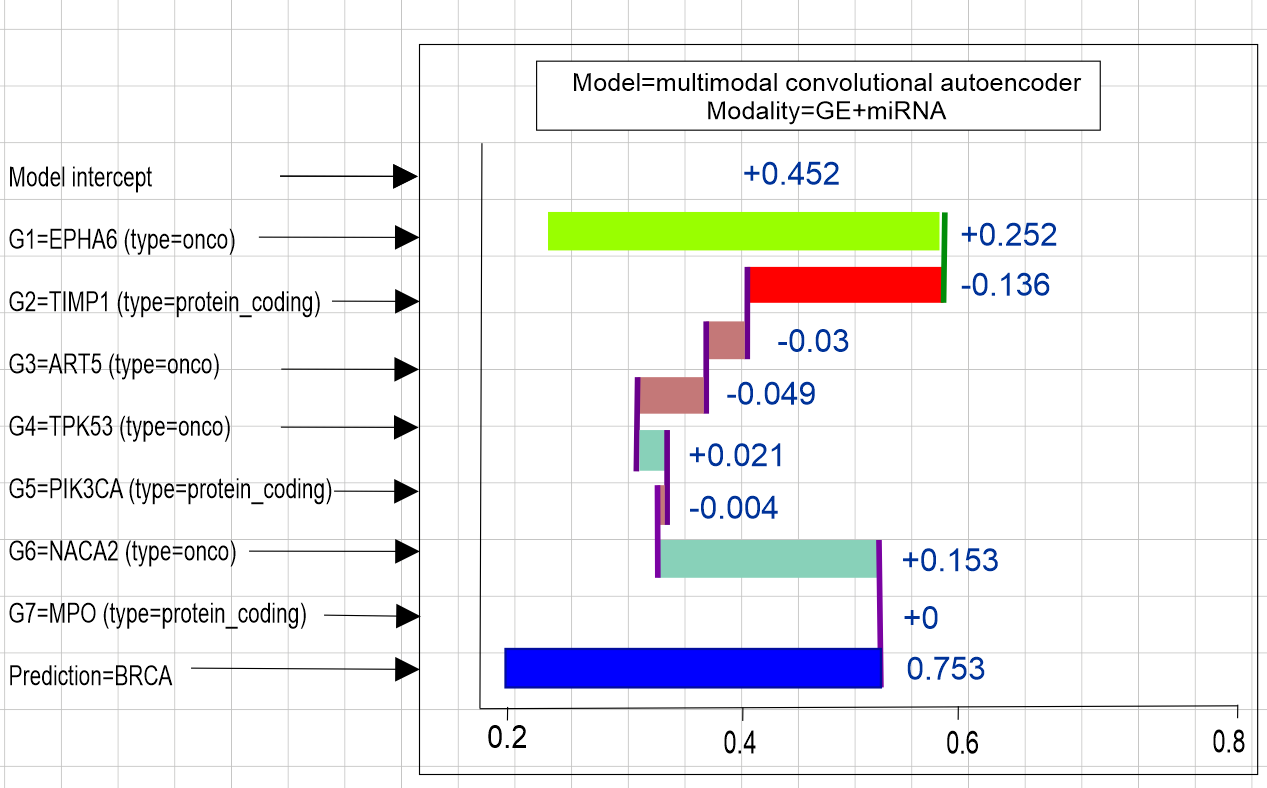
\includegraphics[width=0.5\linewidth]{images/intercept.png}
	    \caption{Explaining a diagnosis decision to patient is difficult unless it is interpreted simpler way}
	    \label{problem_of_xai:1}
\end{figure}

%For instances where humans can confidently predict the behavior of a model, let(human) precision be the fraction in which they are correct(note that this is human precision, not model precision). High human precision is paramount for real interpretability - one can hardly say they understand a model if they consistently think they know what it will do, but are often mistaken. 
\hspace*{3.5mm} Local interpretability approaches mostly provide explanations to describe the local behavior of a model using a linearly weighted combination of input features~\cite{baehrens2010explain}. Although, linear functions can capture relative feature importance, whether they apply to an unseen instance is not clear, given that linear explanations are local. Besides, the coverage\footnote{Coverage w.r.t. rules signifies region where explanation applies} is unclear, which can lead to low human precision~\cite{ribeiro2018anchors}. 
In the previous chapters, we have seen that explaining a diagnosis decision with plots and charts are good for exploration and discovery. We have seen how the models are helpful at predicting cancer types~(diagnosis). However, interpreting them for the first time may be difficult. For example, suppose the multimodal convolutional autoencoder predicts the selected patient has breast cancer in which model's average response~(i.e., intercept) on the GE+miRNA modality is +0.452. The model predicts that the selected patient was diagnosed with a probability of 75.3\%. It also displays all the variables that had contributed to that prediction, but still interpreting it to a patient for the first time may be difficult unless they are explained in a simple human-interpretable decision rule.  

\hspace*{3.5mm} Nevertheless, for a CDSS, a doctor might want to understand the reasons behind any automatic an automatic diagnosis before making the final diagnosis decision. Domain experts may have knowledge that they learned in years of their research and clinical practice, which is what current ML models may fail to utilize~\cite{ming2018rulematrix}. 
%Using rules~(and rules-based systems) to explicate machine learning results creates explainable AI. Many of the far-reaching applications of AI at the enterprise level — deploying it to combat financial crimes, to predict an individual’s immediate and long-term future in health care, for example — require explainable AI that’s fair, transparent and regulatory compliant. %Rules can explain machine learning results for these purposes and others.
%After organizations gain insight into the black box of intricate machine learning models, the best way to explain those results to customers, regulators and legal entities is to translate them into rules that, by their very definition, offer full transparency for explainable AI. Rules can also highlight points of bias in models.
In this chapter, we provide model-agnostic explanations of the predictions by the MCAE-based models we developed in \cref{chapter:xai} based on IF-THEN rules for the reasoning of a model's prediction so that human users can understand. The goal is to answer the following questions: 

\begin{enumerate}[noitemsep]
    \item What knowledge has the model learned?
    \item What knowledge does the model utilize to make a prediction?
    \item How certain is the model for each piece of knowledge? 
    \item Can we reuse the rules to validate the findings to mitigate decision biases? 
\end{enumerate}

\hspace*{3.5mm} The rest of the chapter is structured as follows: \cref{chapter_7:rw} covers some related works on interpretable decision rules and summarize their potential limitations. \Cref{chapter_7:mm} describes the approach of generating explainable decision rules. \Cref{chapter_7:results} demonstrates some evaluation results and discusses key findings of the study.  \Cref{chapter_7:conclusion} provides some explanations of the importance and relevance of the study reported, highlights the limitations and discuss some future works before concluding the chapter.  

\section{Related Work} \label{chapter_7:rw}
Compared to other interpretable options, rules fare well;users prefer, trust and understand rules better than alternatives,in particular rules similar to anchors. Short, disjoint rules are easier to interpret than hierarchies like decision lists or trees. A number of approaches construct globally interpretable models,many based on rules. With such models, the user should be able to guess the model’s behavior on any example (i.e. perfect coverage). However, these models are not appropriate for many domains,e.g. almost no interpretable rule-based system is suitable for text or image applications, due to the sheer size of the feature space, or are just not accurate enough. 

\hspace*{3.5mm} Interpretability, in these cases, comes at the cost of flexibility, accuracy, or efficiency. An alternative is learning a simple interpretable model to imitate the black-box model globally~(e.g. a decision tree or a set of rules, but this may yield low human precision. Simple models are not able to fully capture the behavior of the complex ones, and thus lead users to wrong conclusions, especially since it is not clear when the simple model is faithful.To avoid this,local model-agnostic explanations explain individual predictions (instead of the whole model at once).These methods provide a trade-off: each explanation is easy to understand even for complex models and tasks, but only captures the behavior of the model on a local region of the in-put space. The anchor approach falls within this category~(and thus can explain complex models like translation and VQA),together with many forms of linear explanations.

\hspace*{3.5mm} Rule-based models are composed of logical representations, that is, IF-THEN-ELSE statements which are pervasively used in programming languages. Typical representations of rule-based models include decision tables [43], decision trees [7], and rule sets or decision lists [33]. Among these representations, trees are hierarchical data that have been studied abundantly in visualization research. A gallery of tree visualization can be found on treevis.net [35]. Most related to our work, BaobabView [42] uses a node-link data flow diagram to visualize the logic of decision trees, which inspired our design of data flow visualization in rule lists.However, there is little research on how visualization can help analyze decision tables and rule lists. The lack of interest in visualizing decision tables and rule lists is partially due to the fact that they are not naturally graphical representations as trees. There is also no consensus that trees are the best visual representations for understanding rule-based models. A comprehensive empirical study conducted by Huysmanset al. found that decision tables are the most effective representations, while other studies [2] disagrees. In a later position paper, Freitas summarized a few good properties rules and tables possess that trees do not. Previous studies used pure texts to present rules.  %In our study, we provide a graphical representation of rule lists as an alternative for navigating and exploring proxy models

\section{Methods} \label{chapter_7:mm}
In this section, we discuss our approach in detail, including data collection, preprocessing, network construction, and training, followed by interpreting the network towards biomarkers identification. 

\subsection{Problem statement}
To know the local and global-behaviour of a model, the task is to generate as set of rules that that ``anchors"~(or, covers) the prediction sufficiently, giving entire model's behaviour~\cite{ribeiro2018anchors}. Since we argued that the interpretability provided by the predictor ${F}$ in \cref{chapter:xai} is not sufficiently human-interpretable and globally too complex, we assume it as a `white-box' model\footnote{However, we still assume it a `black-box' model to some extent.}. Let's it is a partially `white-box' model. From a given such model ${F}: X \rightarrow Y$ and an instance $x \in X$, the goal of local model-agnostic interpretability is to explain the behavior of ${F}(x)$ using decision rules, where $X$ is the full dataset and ${F}(x)$ is the individual prediction for $x$. 

\begin{table}[h!]
    \caption{Example of gene expression samples based on oncogenes}
    \label{ge:ancor_example}
    \vspace{-6mm}
    \begin{center}
        \scriptsize
        \begin{tabular}{l|l|l|l|l|l|l|l|l|l}
            \hline
            \rowcolor{Gray}
            \textbf{Type} & \textbf{Gender} & \textbf{Age} & \textbf{Race} & \textbf{TP53} & \textbf{TBX3} & \textbf{MTOR} & \textbf{MPO}  & .. & \textbf{AMBN} \\\hline    
            BRCA (1) & 1 & 55 & American & 0.3195 & -0.2154 & -0.154 & 0.4767  & .. & 0.652 \\\hline
            BRCA (1) & 1 & 49 & Bangladeshi & 0.230 &  -0.552  & 0.715  & 0.924   & .. & 0.552 \\\hline
            BRCA (0) & 0 & 68 & Canadian & -0.240 &  0.252  & 0.350  & -0.642  & .. & -0.985 \\\hline
            BRCA(0) & 0 & 72 & Egyptian & -0.450 &  0.012  & 0.650  & -0.325  & .. & 0.357 \\\hline
        \end{tabular}
        \vspace{-4mm}
    \end{center}
\end{table}

%\hspace*{3.5mm} Providing human-level interpretability by "zooming in" on individual predictions makes the explanation task easier and trustworthy\cite{ribeiro2018anchors}. %Nevertheless, since both perturbations $\mathcal{D}$ and explanations must use an interpretable representation even if the model uses an alternative representation of the input, we employed a model-agnostic method called anchor\cite{ribeiro2018anchors}, which works by perturbing the instance $x$ according to some ``perturbation distribution" $\mathcal{D}$.  

\begin{sidewaysfigure*}
	\centering
		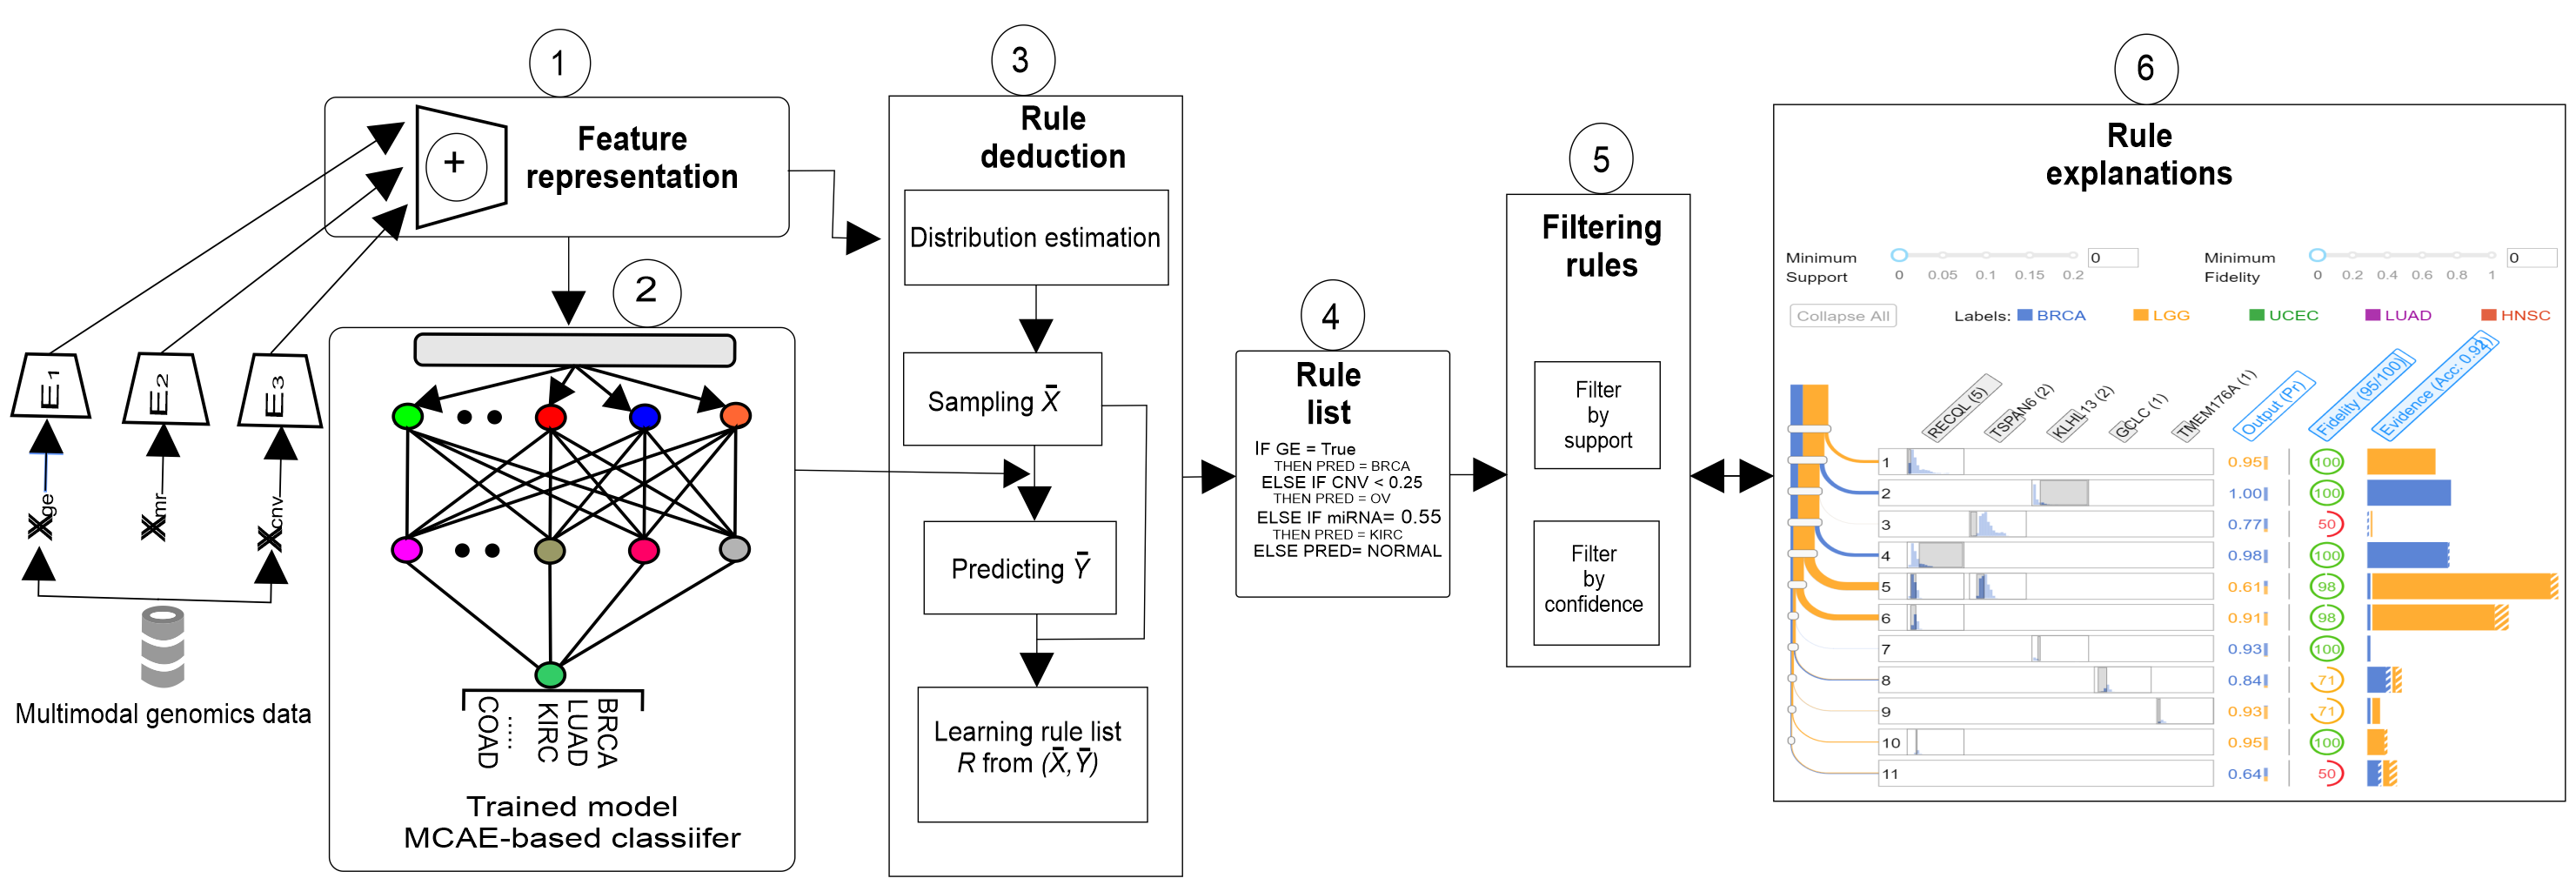
\includegraphics[width=\linewidth]{images/rules_wf.png}
	    \caption{The rule generation and explanation workflow: (1) multimodal genomics data is used to create for learning representation, (2) a model is trained, (3) model produces a rule list by approximating it's behaviour, (4) rule list is filtered based on given support and confidence, before (5) explaining the decision} 
	    \label{fig:rules_wf}
\end{sidewaysfigure*}

\hspace*{3.5mm} Let $R$ be a rule~(in the form of set of predicates) to provide interpretable representation, such that $R(x)$ returns 1 if all its feature predicates are true for instance $x$, 0 otherwise. For example, in \cref{ge:ancor_example} when x=\{1, 0.3195, -0.2154, -0.154, 0.4767, 0.652\} or x=\{1, 0.230, -0.552, 0.715, 0.924, 0.652\}, $F(x)=Y$, $A(x)=1$ where $A=\{TP53, TBX3, MPO, AMBN\}$. On the other hand, when x=\{0, -0.240, 0.252, 0.350, -0.642, -0.985\} or x=\{0, -0.450, 0.012, 0.650, -0.325, -0.357\}, $ F(x)=N$, $R(x)=0$ where $R=\{TP53, TBX3, MTOR, MPO\}$. Representing a decision this intuitive way, however, is not very user friendly given the continuous nature of the data and huge number of protein-coding genes~(i.e., more then 20k). Therefore, we need a better rule list to approximate the behaviour of the original  models trained on dataset $X$. 

\subsection{Generating decision rules}
Our approach is based on RuleMatrix~\cite{ming2018rulematrix}, which is Bayesian rule approach to generate and explain model's decision. The overall workflow is shown in \cref{fig:rules_wf}: first the multimodal genomics data is used to create for learning representation on which a model is trained. Then a surrogate model produces a rule list by approximating original model's behaviour. Since not every rule has better coverage, support, and confidence, filtering can be performed by a user~(a doctor) based on support and confidence before explaining the final decision to another user~(e.g., a patient).\\ 

\vspace{-2mm}
\begin{tcolorbox}[colback=white!3!white,colframe=gray!120!black,title=\faBook~Overlapping rules vs. interpretability:]
    \scriptsize{
        \textbf{Overlapping rules}: rules can overlap. For example, imagine when we want to predict the cancer type of a sample but two or more rules, giving contradictory predictions. Even there is a possibility that even a not a single rule applies. Interpretability suffers potentially when several rules apply~\cite{molnar2019interpretable}. For the former, we can solve using a decision list. \\
        \textbf{Decision list}: it is an order to the decision rules~\cite{molnar2019interpretable}. If the condition of the first rule is true, we rely on the prediction of a DSS based on the first rule. Otherwise, we keep checking the next rule and so on. This way, decision lists can solve the problem of overlapping rules by returning the prediction of the first rule only. \\
        \textbf{Decision set}: it resembles a representativeness of the rules, except that some rules might have a higher voting power. According to set theory, rules are either mutually exclusive, or there is a strategy to resolve the conflicting rules, s.t. weighted majority voting of individual rule accuracies~\cite{molnar2019interpretable}. 
        }
\end{tcolorbox}

\hspace*{3.5mm} Since, we already covered the representation learning and predictive modelling in \cref{chapter:xai}, we will cover only the model surrogate, rule generation, filtering of rules, and rule-based explanation steps. 

\subsubsection{Model surrogation}
A surrogate model is an interpretable model trained to approximate the predictions of the underlying model~(i.e., a `black box' model) as accurately as possible and to be interpretable. In other words, by interpreting the surrogate model, we can draw conclusions about the `black box' model~\cite{molnar2019interpretable}. There is actually not much theory needed to understand surrogate models. We want to approximate our `black-box' prediction function $f$ as closely as possible with the surrogate model prediction function $g$, under the constraint that $g$ is interpretable. 

\hspace*{3.5mm} For $g$, any interpretable model can be used~\cite{molnar2019interpretable}. Since we already have a trained models, training a surrogate model would be easy, as long as we have access to data and prediction function\footnote{It is a model-agnostic method as it does not require knowing inner working principle of the `black-box' model}. If the underlying ML model is replaced with another, the surrogate model will still be usable~\cite{molnar2019interpretable}. \Cref{algo:surrogate_model_generation} outlines the necessary steps to obtain a surrogate model:

%\vspace{-2mm}
\begin{algorithm*}[h]
\caption{Generating surrogate model}
\small{
    \DontPrintSemicolon \SetKwInOut{Input}{Input}%
    \SetKwInOut{Output}{Output}%
    \Input{Dataset $X$ for training the `black-box' model $M_b$ or a new dataset from the same distribution for training the surrogate model, interpretable model type $t$ and params $p$.}%
    \Output{A surrogate model $M_s$ and predictions $Y_s$ to approximate `black-box' model $M_b$.}%
    \BlankLine%
    \For{for each sample $x \in X$}{\tcp*{For dataset $X$, get  predictions for black box model $M_b$}
        \vspace{-2mm}
        $Y_b \leftarrow  M_b.predict(X)$\;
        \textbf{Return} $Y_b$  
    }
    \BlankLine%
    \For{for each sample $x \in X$}{\tcp*{for each sample in training set do}
        \vspace{-2mm}
        $M_s \leftarrow  \{\}$\;
        $Y_s \leftarrow  \{\}$\;
        $t \leftarrow  \{\}$\; \tcp*{e.g., linear model, decision tree}
        %\vspace{-2mm}
        $clf \leftarrow  estimatorInstantiate(t,p)$\;\tcp*{Instantiate an interpretable estimator}
        \vspace{-2mm}
        $M_s \leftarrow  clf.fit(X, Y)$\; \tcp*{train the interpretable model $M_s$ on dataset $X$}
        \vspace{-2mm}
        $Y_s \leftarrow  M_s.predict(X)$\; \tcp*{Get the predictions of the surrogate model}
        \textbf{Return} $[(M_b, Y_b)(M_s, Y_s)]$
     }}
     \label{algo:surrogate_model_generation}
\end{algorithm*}

\hspace*{3.5mm} R-squared measure~($R^2$) is a way to measure how well the surrogate replicates the `black-box' model~\cite{molnar2019interpretable}. The $R^2$ can be measured mathematically, as follows~\cite{molnar2019interpretable}: 

\begin{equation}
    R^{2}=1-\frac{SSE}{SST}=1-\frac{\sum_{i=1}^{n}\left(\hat{y}_{*}^{(i)}-\hat{y}^{(i)}\right)^{2}}{\sum_{i=1}^{n}\left(\hat{y}^{(i)}-\overline{\hat{y}}\right)^{2}}
    \label{ew:r_squared}
\end{equation}

\hspace*{3.5mm} where $\hat{y}_{*}^{(i)}$ is the prediction for the $i^{th}$ instance of the surrogate model $M_s$, $\hat{y}^{(i)}$ is the prediction of the `black-box' model $M_b$, $\overline{\hat{y}}$ the mean of the `black-box' model predictions, $SSE$ is the sum of squares error, and $SST$ is the sum of squares total~\cite{molnar2019interpretable}. The $R^2$ can be interpreted as the percentage of variance captured by the surrogate model, as follows~\cite{molnar2019interpretable}:

\begin{itemize}[noitemsep]
    \item If $R^2$ is close to $1(=$ low $\mathrm{SSE}$), then the interpretable model approximates the behavior of the `black-box' model very well\footnote{In such scenario, we even can replace the complex model with the interpretable model.}. 
    \item If $R^2$ is close to 0~(i.e., high SSE), the interpretable model will fail to explain the `black-box' model\footnote{In such scenario, we should not replace  complex model with the interpretable model.}. 
\end{itemize}

\subsubsection{Rule set generation}
Similar to literature~\cite{ming2018rulematrix}, we apply the representation of an ordered list of inclusive rules based on Bayesian rule lists. Based on a partially `white-box' model ${F}$, the task is to extract a rule list $R$ to explain it's decision. However, as shown in \cref{fig:rules_wf}, we treat the original~(trained) model as a teacher that have sufficient knowledge and the student model is trained using the data ``labeled" by the teacher, s.t. the predictions of the teacher model is used as ground truth instead of the real ones. RuleMatrix takes a trained model ${F}$~(i.e, teacher) and training set $X$ as input to produce a rule list $R$ generated through a surrogate model by approximating the classifier  w.r.t, fidelity as the accuracy with the true labels as the output of ${F}$~\cite{ming2018rulematrix}. On the other hand, we measured the performance of the surrogate model itself using $R^2$ to measure how well the surrogate replicates the `black-box' model.    

\vspace{-6mm}
\begin{align}
    \text {fidelity}(R)_{{X}}=\frac{1}{|{X}|} \sum_{\boldsymbol{x} \in {X}}[F(\boldsymbol{x})=R(\boldsymbol{x})],
    \label{eq:fidelity}
\end{align}

\hspace*{3.5mm} where $F(\boldsymbol{x})=R(\boldsymbol{x})$ is 1 if $F(\boldsymbol{x})=R(\boldsymbol{x})$, 0 otherwise. Technically, a student model is necessarily a `surrogate model' - a simplified version of the teacher model, which maps $Y_\text{sample}=F(X_\text{sample})$ to approximate the original model $F$~\cite{forrester2008engineering}. Then in context of Bayesian statistics, we want to optimize a function $Y=F(x)$, which is, however, very expensive to evaluate. Instead, we one optimize the surrogate model $Y_\text{sample}=F(X_\text{sample})$, which is faster to evaluate and we assume will reasonably represent the original model $F$ behaviour. Hence, this is an optimization problem, where the objective is to maximize the fidelity of the rule list~\cite{ming2018rulematrix}. Since we have access to both a trained model and the data used to train the model, estimating the distribution of the training data ${X}$ is feasible. Unlike literature~\cite{ming2018rulematrix}, we don't require the joint distribution estimation~(i.e., for discrete and continuous features), given that our feature space is continuous. We create sample ${X}_{\text {sample}}$\footnote{Where the number of samples is a customizable parameter set by human, e.g., data scientist} based on the original model $F$ predicts the labels. Finally, the sampled data ${X}_{\text {sample}}$ and the labels ${Y}_{\text {sample}}$ are then used to generate the rule list.

\hspace*{3.5mm} Since the classifier $F$ can reach it's decision through multiple rules with excessive length, applying sequential covering\footnote{A general procedure that repeatedly learns a single rule to create a decision list or rule set~\cite{molnar2019interpretable}} the entire dataset rule by rule was not what we optimally think. Therefore, depending upon the length of number of predictors~(i.e, features), RuleMatrix adopted the Scalable Bayesian Rule List~(SBRL) algorithm proposed by Yanget al.~\cite{BayesianRule}. In SBRL, pre-mined frequent patterns are combined into a decision list using Bayesian statistics~\cite{molnar2019interpretable}. 
This is also align with our case given that the training set has a large number of features. Nevertheless, since we are trying to solve a multiclass classification problem, we extend the output distribution of RuleMatrix to multinomial instead of binomial. On the other hand, since a very long rule is not easily interpretable, RuleMatrix uses the minimum description length binning~(MDLB)\footnote{\url{https://github.com/hlin117/mdlp-discretization}} discretization to discretize the features and the FP-Growth frequent mining algorithm to get the candidate rule sets based on which the final rule set is generated. In our approach, however, MDLB was not a feasible option due to the nature of the data. Therefore we come up with our own discretization based on domain knowledge.

\hspace*{3.5mm} SBRL algorithm expects all the input features to be categorical, while our data set has a bunch of continuous features. In such a case, discretization could help not only to get better accuracy~\cite{maslove2013discretization} but also help interpreting the decision rules better. This means that we have to represent the features to be categorical such that numeric features have to be categorized. There are many ways to cut a continuous feature into intervals, but this is not trivially straightforward way. Now question is how many intervals should the feature be divided into? Maybe we could employ two splitting criteria such as quantiles and fixed interval lengths. For the former, we can binning continuous features based on the frequency of the values by quantiles is an option. However, that's a tricky part and would give so many bins that would not help us in interpreting a rule. On the other hand, although genomics data we use are also mostly continuous, domain expertise or knowledge might help. For example, according to baseline expression results, we discritized gene and miRNA expressions into 4 different levels\footnote{\url{https://www.ebi.ac.uk/gxa/FAQ.html}}:

\vspace{-2mm}
\begin{itemize}[noitemsep]
    \item \textbf{Below}: if expression level is less than the cutoff~(0.5 FPKM\footnote{FPKM: Fragments Per Kilobase Million- is a normalised estimation of gene expression based on RNA-seq data.}).
    \item \textbf{Low}: if expression level is between 0.5 to 10 FPKM.
    \item \textbf{Medium}: if expression level is between 11 to 1000 FPKM. 
    \item \textbf{High}: if expression level is higher than 1000 FPKM. 
\end{itemize}

\hspace*{3.5mm} In many cases, CNVs can encompass genes leading to imbalances, e.g., genes that were thought to always occur in 2 copies per genome have now been found in 1, 3, or more than 3  copies\footnote{\url{https://www.gene-quantification.de/cnv.html}}. This findings also reflected in our data. Based on this assumption, we use the segmentation mean as the basis for computing the change in numeric values and discritized CNV features into 3 different levels:  

\vspace{-2mm}
\begin{itemize}[noitemsep]
    \item \textbf{Normal}: if CNV with exactly 2 copies.
    \item\textbf{Low}: if CNV with low number of copy because of deletion that range between -4 and 1, i.e., less than normal copies.
    \item\textbf{High}: if CNV with high number of copy because of copy number gain that range between 3 and 4~(in rare case between 3 and greater than 4) than normal copy~(i.e., 2).
\end{itemize}
\vspace{-2mm}

\hspace*{3.5mm} As already stated in \cref{chapter:preli} that a decision rule is a logical statement consisting of two parts called the antecedent~(IF) and the consequent~(THEN), where antecedents can have multiple AND and OR clauses. However, similar to RuleMatrix, we restrict the antecedent to be a conjunction~(i.e., AND) of clauses, where each clause is a condition on an input feature, which eases users' cognitive burden of discriminating different logical operations. Eventually, the output of each rule is a probability distribution over the classes, representing the probability of an instance satisfying the antecedent belongs to each class. However, for a better understandability, we show the highest probabilities of two probable classes only. 
%The simplest way to present a rule is to write it down as a logical expression, which is ubiquitous in programming languages. 

\subsubsection{Filtering rules}
%In contrast, even though LIME uses the same $\mathcal{D}$, anchors adapt their coverage to the model's behavior and makes their boundaries clear. 
% Anchors are intuitive, easy to comprehend, and have extremely clear coverage – they only apply when all the conditions in the rule are met, and if they apply the precision is high. 
However, we found textual representations difficult to navigate when the length of the list is too large, given that our feature space is too large. Nevertheless, in textual representations, the input features do not necessarily represent in the same order in each rule, making it  difficult for users to search a rule with certain filtering criteria or when comparing conditions used in other rules. 
Further, the filtering of rules helps relieve the scalability issue and reduce the cognitive load when the extracted rule list is too long. This is very crucial for our case, since our teacher models are very complex model and trained on high dimensional multimodal genomics data. 
When performing inference, each rule is queried in order and will only fire if all its previous rules are not satisfied. This allows fast queries and bypasses the complex conflicts resolution mechanisms~\cite{ribeiro2018anchors}.

\hspace*{3.5mm} Therefore, to check if a rule list approximates the model reasonably well, we provide two types of filters: filter by support and filter by confidence. The former filters out the rules that have little support, assuming those are not useful explaining clinical decisions. The latter filters out rules that have low confidence, making them insignificant in discriminating different classes while explaining clinical decision. Apart from the overlapping and conflicting rules, there is no better way to justify if the generated explanations justify how faithful they are, i.e., what their ``coverage" is. 

%\subsubsection{Challenges} 
%Ambiguities: i) many biomarkers, e.g., genes have different names (e.g., synonym) across sources, ii) describing the prediction in natural language.

%Inconsistencies across reasoner: i) different reasoner, e.g., HermiT, Pallet, Fact++, ELK, TrOWL may produce slightly different axioms.
%\subsection{Inference and rule-based explanation}

\section{Experiments} \label{chapter_7:results}
In this section, we discuss the evaluation results, both quantitatively and qualitatively. Besides, a comparative analysis with state-of-the-art approaches is provided. 

\subsection{Experiment setup}
We evaluate RuleMatrix explanations for the models we trained in \cref{chapter:xai} on a number of tasks, primarily focusing on how they facilitate accurate predictions by users on the behavior of the models on unseen instances. 
%All the programs were written in Python. The software stack consists of scikit-learn, LIME, and Keras with TensorFlow backend. The network was trained on an Nvidia GTX 1080i GPU with CUDA and cuDNN enabled. 
Accuracy of the rules are reported in macro-averaged precision and coverage metrics that are produced with random search of hyperparameters and 10-fold cross-validation tests. The rule list is visualized with the training data and a rule filter of minimum evidence and support are changed interactively, giving the end user the freedom of filtering rules. 

\subsection{Analysis of rule coverage and confidence}
The overall performance based on RuleMatrix is demonstrated in \cref{table:rules_overall_result}. We report the mean fidelity in percentage. In parenthesis, we the show standard deviations. For the demonstration purpose, we consider the fidelity levels 80\% as high, 60\% to 80\% as medium, and below 60\% as low, respectively. As shown, the worst mean accuracy and confidence of $F_1$ for 10 runs reached 83.21\% and 82.32\% on the CNV test set, with a standard deviation of 2.6\% and 2.2\%. While model $F_2$ performs slightly better on the same modality giving 86.16\% and 85.37\%, with slightly lower standard deviations of 1.7\% and 1.5\%. Thus, both models give low accuracy, albeit model $F_2$ generates slightly better decision rules. 

\begin{table}[h!]
    \centering
    \caption{The mean fidelities of the rule list generated by RuleMatrix based on $F_1$ and $F_2$.}
    \label{table:rules_overall_result}
    \vspace{-2mm}
    \scriptsize{
    \begin{tabular}{l|l|l|l|l} 
        \hline
         & \multicolumn{2}{c|}{$F_1$} & \multicolumn{2}{c}{$F_2$} \\ 
        \hline
        \textbf{Modality} & \textbf{Fidelity} & \textbf{Confidence} & \textbf{Fidelity} & \textbf{Confidence} \\ 
        \hline
        GE  & 89.25~(2.5) & 87.54~(2.1) & 91.27~(1.42) & 89.33~(1.25) \\ 
        \cline{1-3}\cline{4-5}
        CNV & 83.21~(2.6) & 82.32~(2.2) & 86.16~(1.7) & 85.37~(1.5) \\ 
        \hline
        miRNA & 87.54~(1.9) & 86.63~(1.7) & 88.35~(1.45) & 87.55~(1.85) \\
        \hline
    \end{tabular}}
    \vspace{-4mm}
\end{table}

However, for miRNA modality, we experience relatively better accuracy and confidence: we recorded 87.54\% and 86.63\% mean accuracy and confidence from $F_1$ for 10 runs, with a standard deviation of 1.9\% and 1.7\%. While model $F_2$ performs slightly better on the same modality giving 88.35\% and 87.55\%, with slightly lower standard deviations of 1.45\% for fidelity but slightly higher standard deviations of 1.85\% for confidence. This means both models give better accuracy, albeit we can't confidently say that $F_2$ helps generate better decision rules, even though it gives better accuracy. 

\hspace*{3.5mm} On the other hand, overall the best mean accuracy and confidence of $F_1$ for 10 runs reached 89.25\% and 87.25\% on the GE test set, with a standard deviation of 2.5\% and 2.1\%. While model $F_2$ outperforms model $F_1$ on the same modality giving 91.27\% and 89.33\%, with slightly lower standard deviations of 1.42\% and 1.25\%. This means model $F_2$ not only gives better accuracy but also generates relatively stable and reliable rules. The best model $F_2$ significantly outperforms model $F_1$ on gene expression data. Consequently, we explain the predictions to end users with decision rules generated by model $F_2$ on gene expression modality in subsequent sections. 

\subsection{Effects of sampling rate on rule list length and fidelity}
We study the effect of sampling rate on rule list length over three different but single modalities: gene expression, miRNA expression, and copy numbers. We perform 10-fold cross-validation, such that each experiment performed 10 times to compute the fidelity on the test set. As shown in \cref{fig:lr_vs_length}, fidelity of the extracted rule lists on all the modalities generally increases with the increased sampling rate except when the same started declining for the `copy numbers' modality when we set the sampling rate to 5.0. On the other hand, as seen, we experience highest fidelities for the `gene expression' modality. In contrast, moderately high fidelities were recorded for the 'miRNA expression' dataset, making `copy numbers' not suitable for generating and explaining diagnosis decision based on it. 

\begin{figure*}[h!]
	\centering
	\begin{subfigure}{.48\linewidth}
		\centering
		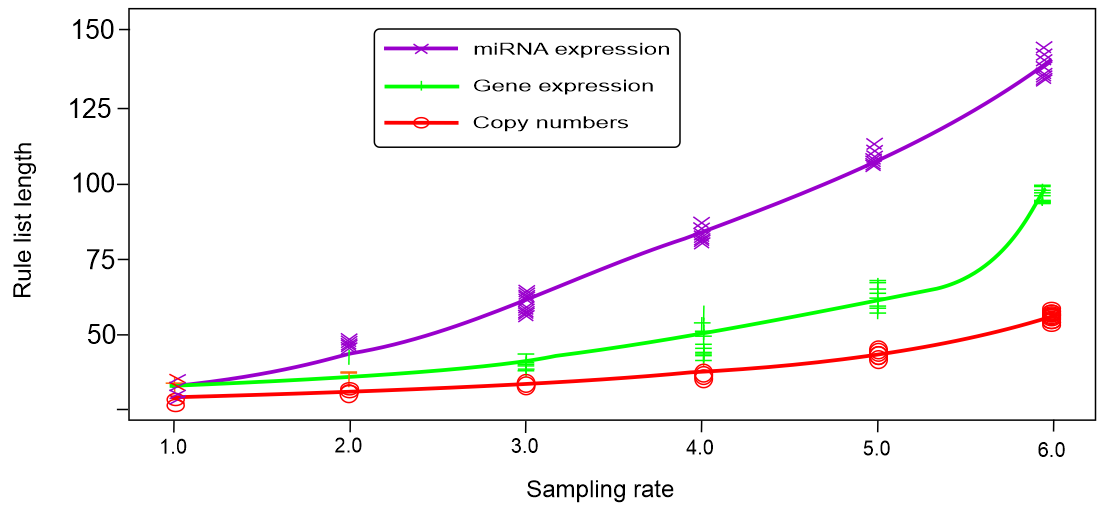
\includegraphics[width=0.8\linewidth,height=40mm]{images/sr_vs_ll.png}
		\caption{Sampling rates vs. rule list length}
        \label{fig:lr_vs_length}
	\end{subfigure}
	\begin{subfigure}{0.48\linewidth}
		\centering
		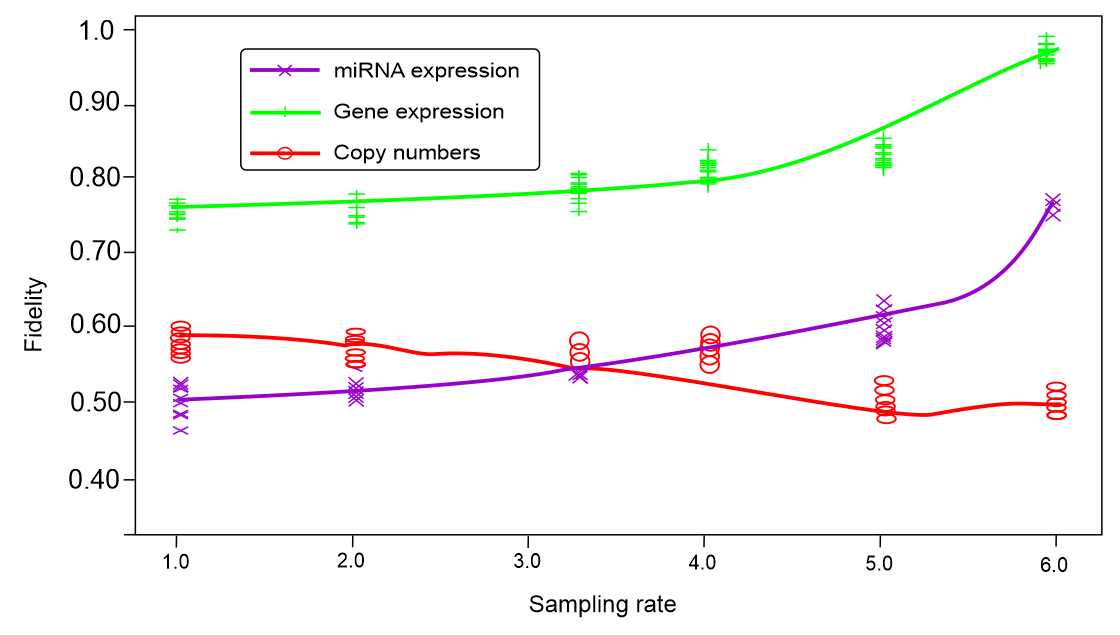
\includegraphics[width=0.8\linewidth,height=40mm]{images/sr_vs_fide.png}
		\caption{Sampling rates vs. fidelity}
        \label{fig:lr_vs_fidelity}
	\end{subfigure}
	\caption{The effect of sampling rates on rule list length and fidelity for different single modality} 
	\label{fig:lr_vs_length_and_fidelity}
\end{figure*}

%\subsection{Effect of sampling rates on fidelity}
\hspace*{3.5mm} We study the effect of sampling rate on rule list length over three different but single modalities: gene expression, miRNA expression, and copy numbers. 
%We perform 10-fold cross-validation, such that each experiment performed 10 times to compute the fidelity on the test set. 
As shown in \cref{fig:lr_vs_fidelity}, fidelity of the extracted rule lists on all the modalities generally increases with the increased sampling rate except when the same started declining for the `copy numbers' modality when we set the sampling rate to 5.0. On the other hand, as seen we experience highest fidelities for the `gene expression' modality. In contrast,  moderately high fidelities were recorded for the 'miRNA expression' dataset, making `copy numbers' not suitable for generating and explaining diagnosis decision based on it. 

\hspace*{3.5mm} As shown in \cref{fig:lr_vs_fidelity}, with all three datasets, the fidelity of extracted rule lists generally increases as the sampling rate grows. At the same time, the complexity of the rule lists also increases drastically, exposing a trade-off between the fidelity and interpretability of the extracted rule list. Considering interpretability is our goal, we follow an intuitive strategy for choosing optimal sampling rate. We  start from a small sampling rate of 1.0, and gradually increase it until we get a good fidelity~(as shown in \cref{fig:lr_vs_fidelity}) or the length~(as shown in \cref{fig:lr_vs_length}) of the rule list exceeds an acceptable threshold. As shown in~\cref{table:rules_overall_result}, our approach generates rule lists that approximate model $F_2$ better with high fidelity on gene expression and acceptable on miRNA expression dataset. 

\subsection{Explaining decisions with rules}
We explain both global and local behaviours of the model~($F_2$) trained on the gene expression dataset. We employ `RuleMatrix', `Skater', and `SHAP' for explaining the decisions both globally and locally. However, SHAP is used in \cref{chapter:fairness} to improve the fairness given their underlying implementation structures. A particular advantage of Skater' is that it can be used to plot the decision generated by the surrogate model in the form of decision trees. 

\subsubsection{Explaining global behaviour}
The data flow in \cref{fig:decision_rules_explain}, shows how all the gene expression data is captured by each of the rules. The width of the flow indicates the number of data captured and uncaptured by each rule, while the color of the flow indicates different labels. In the right of the matrix shows the fidelity and evidences. Fidelity means how accurate a rule is in approximating the $F_2$ model on the gene expression data captured by this rule. 
As stated in \cref{eq:fidelity}, fidelity ranges between 0 and 1. Hence, we plot the fidelity of the rule between 0 to 100 scale to on the subset of data satisfying the rule. As fidelity represents how accurately the rule represents the original model on this subset~\cite{ming2018rulematrix}, the higher the fidelity, the more reliable the rule is in representing the original model. The evidence or support signifies the number of data with different labels. For example, the data captured by rule 2, 3, 4, 7, 8, and 11 represent breast cancer cases. The stripped part encodes the part of data wrongly classified by the model as a certain label represent by the color.

\begin{sidewaysfigure}
	\centering
	\captionsetup{justification=centering}
		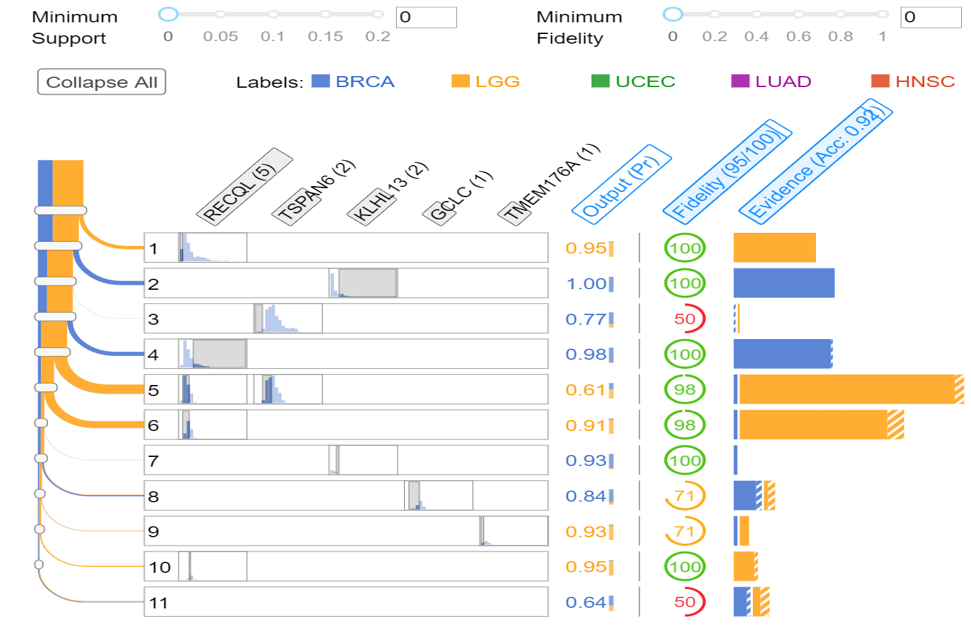
\includegraphics[width=0.6\textwidth,height=60mm]{images/decision_rules_explain.png}
	    \caption{The rule matrix presents each rule as a row and each feature as a column,\\ where clauses are visualized as glyphs in the corresponding cells. The support\\ slide-bar shows the fidelity of the rule for the sampled data, whereas the\\ evidence signifies model's predictions and errors under a certain rule.}
	    \label{fig:decision_rules_explain}
\end{sidewaysfigure}

\begin{figure}
	\centering
		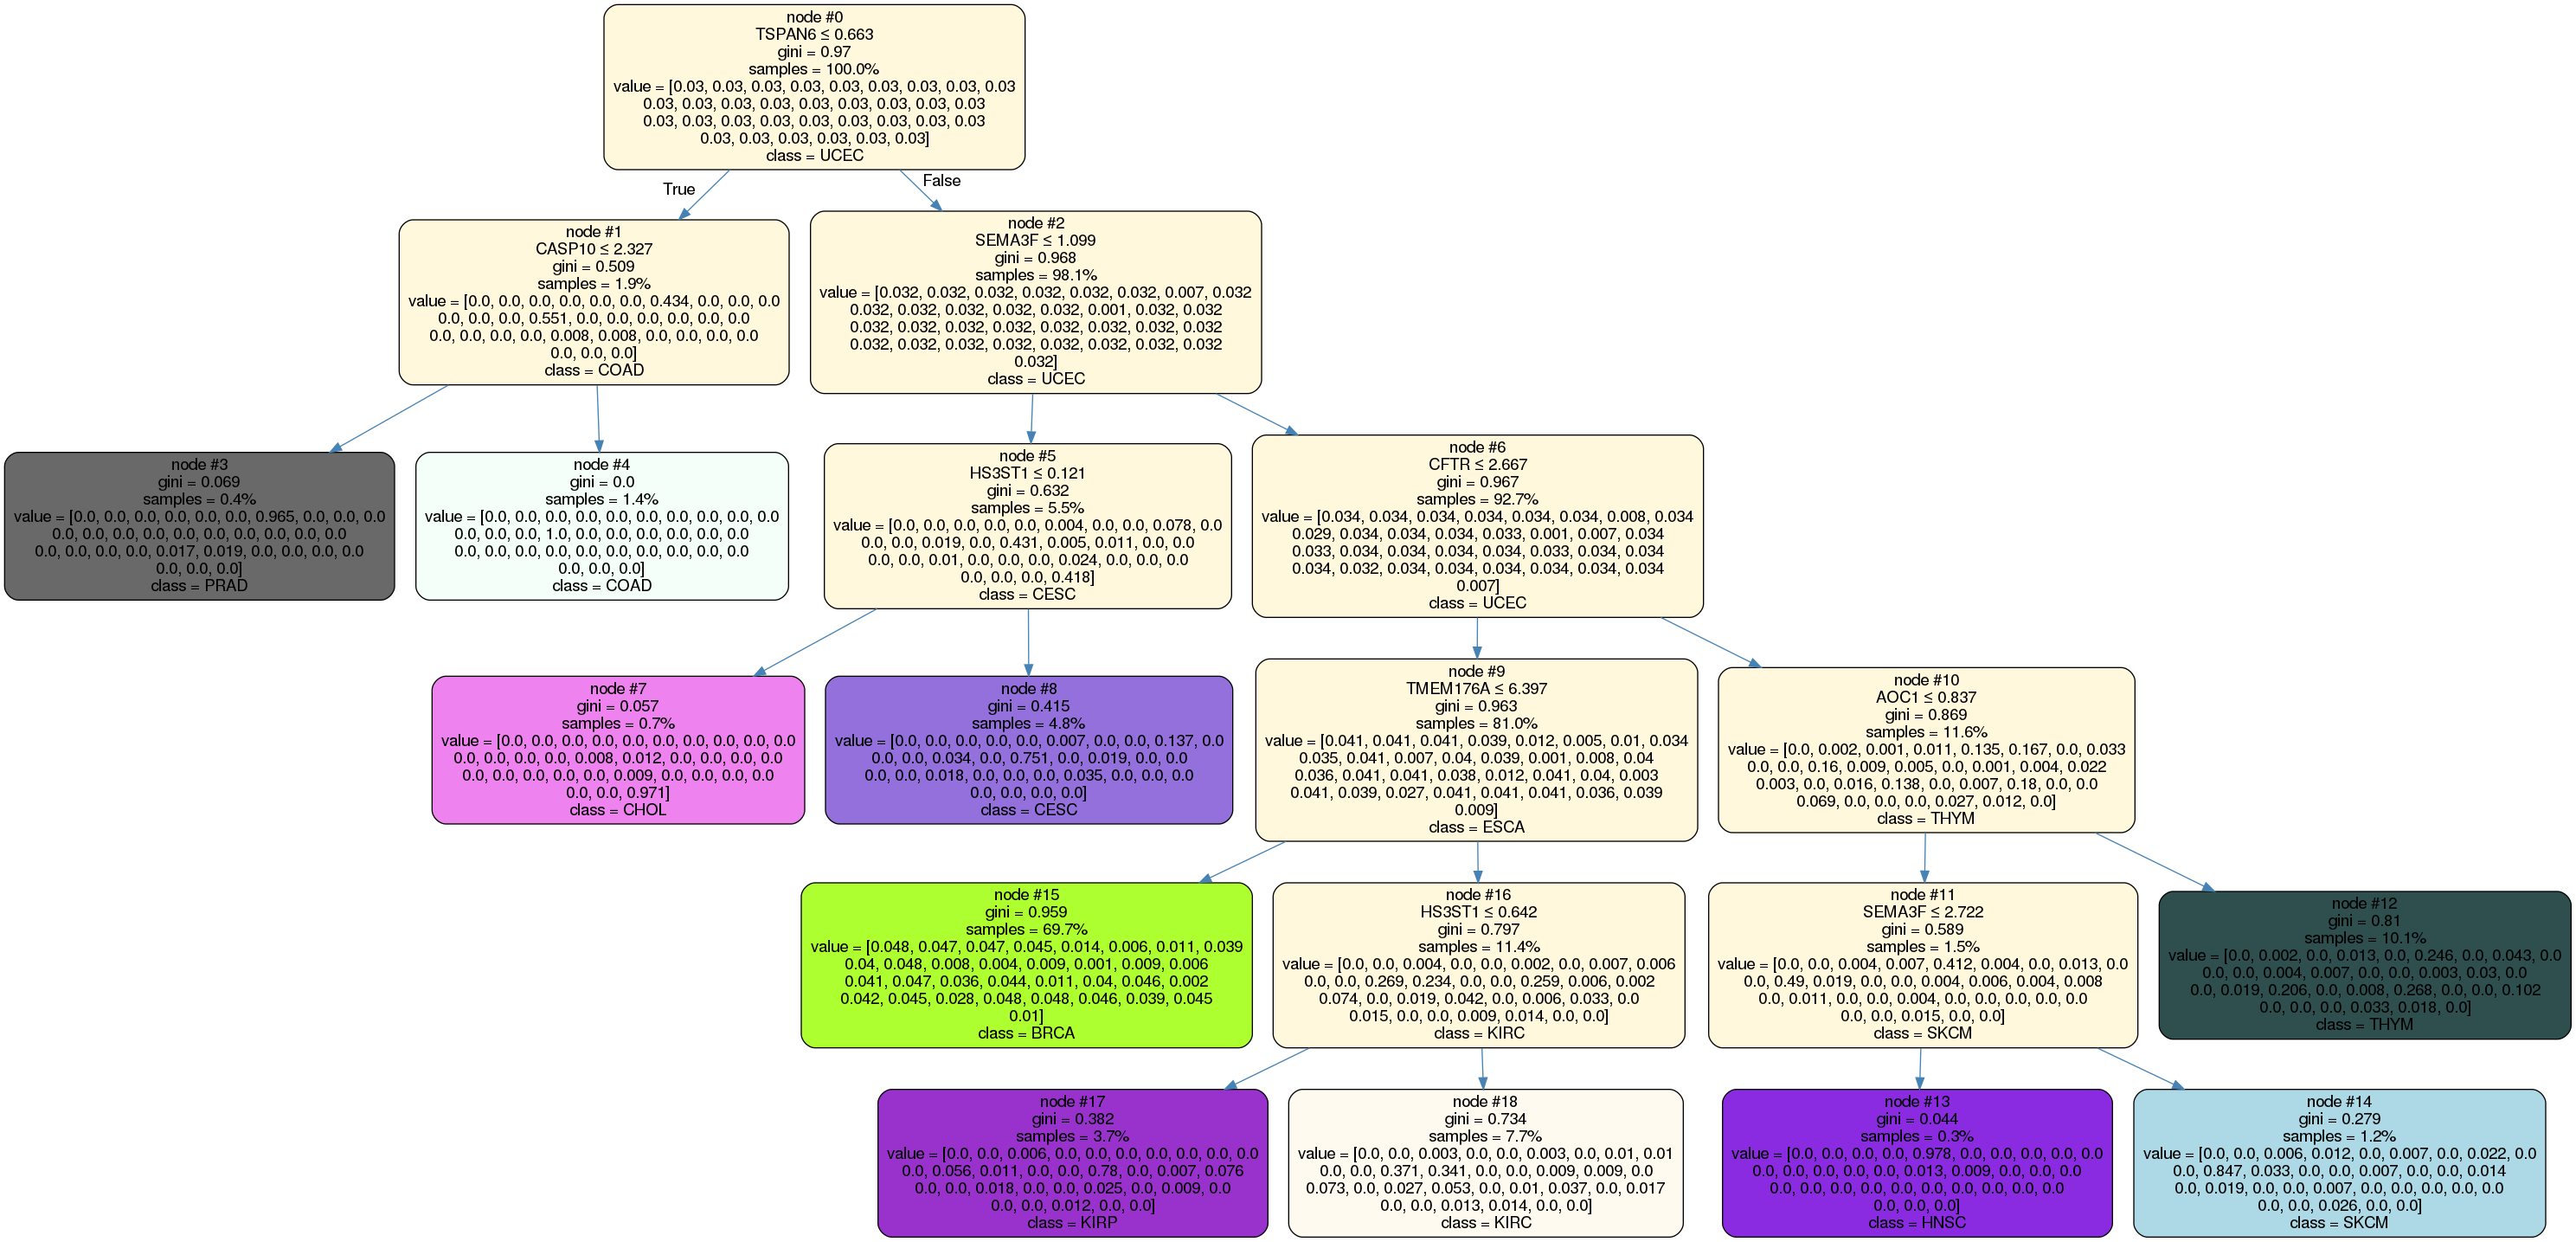
\includegraphics[width=\textwidth]{images/simple_tree_pre.png}
	    \caption{Decision tree showing global decision and explanation.}
	    \label{fig:skater_global}
\end{figure}

\hspace*{3.5mm} We plot the evidence w.r.t., error distribution of the model on  test set of each single modality. The horizontally stacked boxes are used to present the predictions of the model. The width of a box encodes the amount of data with a certain type of predictions. The striped boxes represent erroneous predictions, i.e., wrongly classified  sample as class blue and has true labels different from class blue. To demonstrated an example, a end user extracts a list of 10 rules from the trained model, where the default support was set to 0.1. Subsequently, he observes that rule 3 to 6 do not have enough support from the training data. Hence, he can filter the minimum evidence in the rule filter to 0.05 to collapse the last 5 rules~(rules 6 to 10). Then he finds that the first rule outputs LGG~(i.e., brain lower grade glioma) with a high probability~(i.e., 0.95) and a high fidelity~(i.e., 0.95). 

\hspace*{3.5mm} Based on this rule matrix, he can thn learn that if the marginal adhesion score is larger than 5, the model will very likely predict brain lower grade glioma. This aligns with his knowledge that the loss of adhesion is a strong sign of cancer cells. Then he can check other rules, for example rule 2, which has the largest support from the dataset. The rule shows that if the bland chromatin is smaller or equal than 1, the cell should be kidney cancer. He then should finds this rule interesting since it indicates that one can quickly identify benign cells in the examination by checking if the nucleus is coarse. 

\begin{figure}
	\centering
		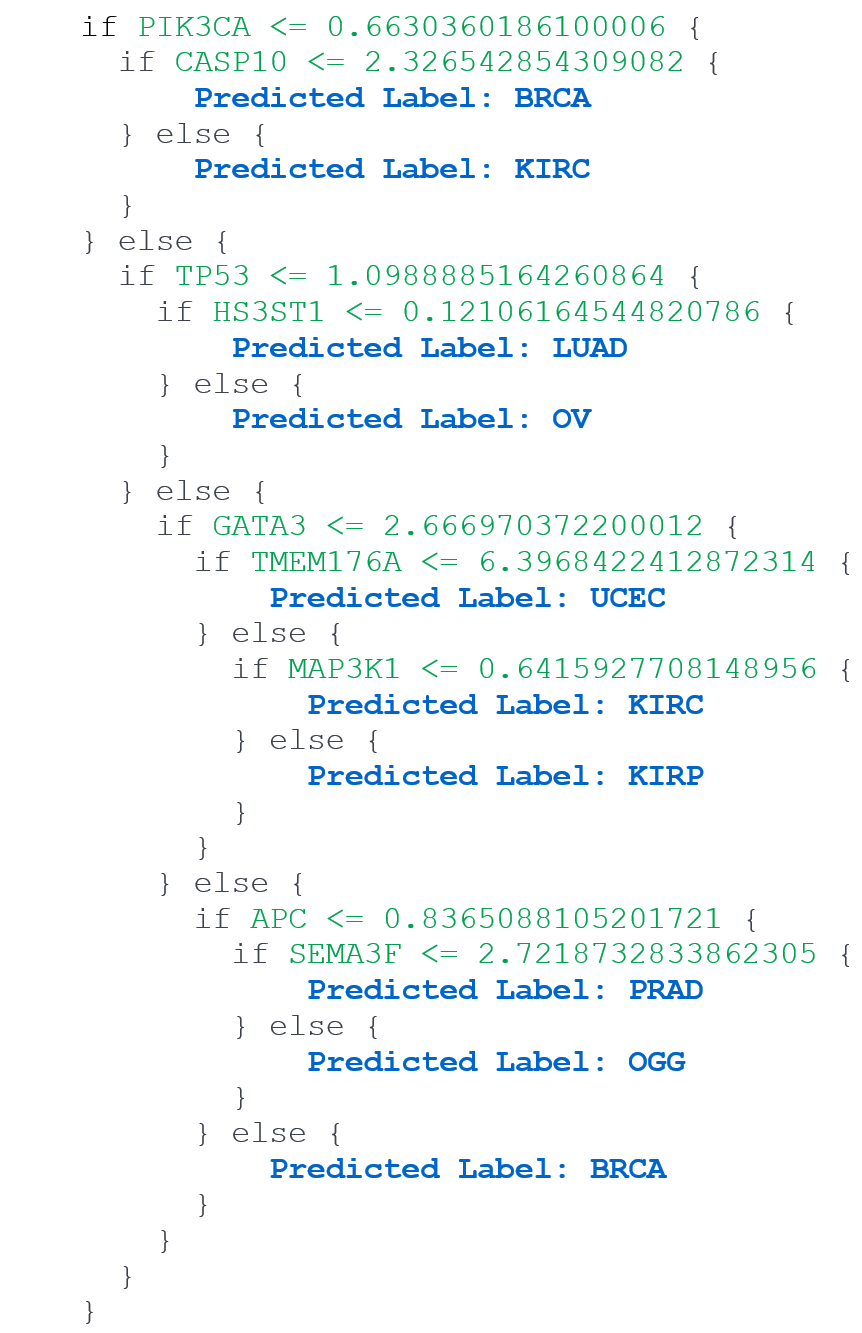
\includegraphics[width=0.4\textwidth,height=90mm]{images/dr_global_1.png}
	    \caption{Global decision as text based on pruned tree}
	    \label{fig:skater_decision_as_text}
	    \vspace{-2mm}
\end{figure}

\begin{figure}
	\centering
		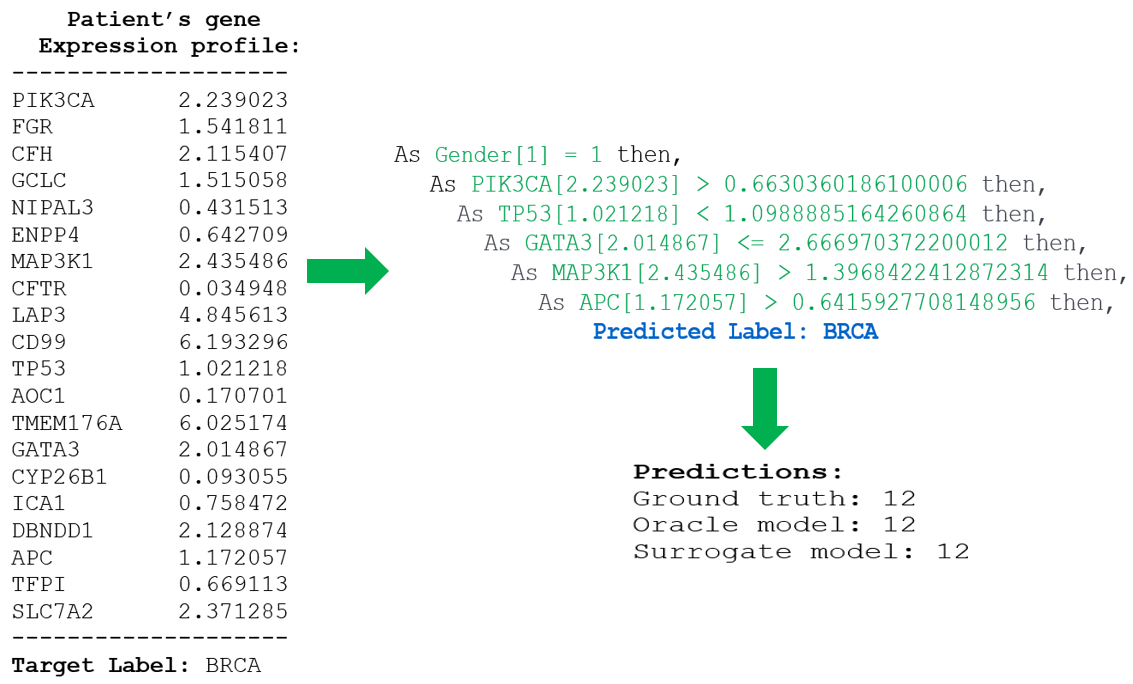
\includegraphics[width=0.8\textwidth]{images/single_pred_feature.png}
	    \caption{Local prediction for a single instance, left: 20 features of the supplied input sample, right bottom: ground truth and the predicted labels by the oracle and the surrogate models}
	    \label{fig:decision_as_text_local_1}
\end{figure}

\hspace*{3.5mm} \Cref{fig:skater_global} shows the global inference tree on the basis of the complete gene expression data set, where only the leaf nodes containing the respective class labels are colored~(gray, pink, purple, dark purples, green, etc.). As seen, the decision tree clearly explains how the model makes the diagnosis decision, which is already better than other charts such as feature importance and partial dependency plots, especially for the exploration and discovery. However, interpreting and explaining them to patients might be still difficult. Therefore, we use Skater to draw the global decision as text based on pruned tree in \cref{fig:skater_decision_as_text}. %The full tree for the same inferencing can be found in appendix. 

\subsubsection{Explaining local behaviour}
Providing human-level interpretability by ``zooming in" on individual predictions makes the explanation task easier and trustworthy\cite{ribeiro2018anchors}. When it comes to explain explaining a decision locally, we plot the decisions as text with 'Skater' by defining the scope to `local'. As seen for a single instance, both the oracle and surrogate models say that the female patient probably has breast cancer, which is based on the fact that several markers genes have contributed. 

\hspace*{3.5mm} Besides, we show how much the respective expression values for these features deviated from their base value predicted by the oracle model trained on the training set. We show the features~(only 20 features are shown for the simplicity) in the left that the mostly focused on to came up with a decision of breast cancer. We already provided the pathway enrichment analysis in \cref{chapter:xai} that also support this findings.  

\subsection{Analysis of missclassified instances}
One of the first steps towards improving an XAI system is to understand it’s weaknesses. However, weakness analysis on black-box models is not straightforward than on models which are interpretable. The better we understand what our models explain why a model works or fails in certain cases and which factors caused it to make a given prediction, the easier it becomes to improve them. Therefore, we put a close focus on the misclassified instances try to analyse the reason behind the wrong predictions. 
We further evaluate the trained model to investigate the reasons behind the incorrect predictions. The trained model~(surrogate) is being evaluated on the test set with 1,200 samples. Since, we had huge feature space, we can't confidently say the model is humanly interpretable, rather output represented as decision stumps based on significant input features, albeit we still say our model is interpretable to major extent. 

\hspace*{3.5mm} After evaluating input data at those indices, we observed that the predicted results are indeed mismatched, giving false positives or false negatives. Since, the model is interpretable, we can infer the cause of incorrect predictions with some efforts. After looking for specific misclassified instances, we found the model implies that if a patient is a male then the likelihood of his BRCA is 95\%. Since the patient in question is a male we can guess the reason behind the false positive, i.e., gender is not an important feature for male patients, while other decision rules are not contributing to the evaluation. Further, we found that both the oracle and surrogate model's predictions were the same for most of the sample examined, which is about 90\% cases, contributing about 10\% contradictory predictions. A more detailed analysis of biological signaling pathways as well as domain validation are further required to validate these findings. 

\subsection{Discussion} \label{chapter_8:discussion}
An intrinsic limitation of the rule induction algorithm results from the trade-off between the fidelity and interpretability of the generated rule list. Depending on the complexity of the model and the focus of specific cancer types for which we want to make diagnostic decision, the algorithm would require a large number of rules in a rule list for the better  approximation of the model with an acceptable fidelity. The interpretability of rules also depends on the meaningfulness of the input features. Since our feature space is huge, this particularly limits the effectiveness of the model. 

\hspace*{3.5mm} Another reason for this is number distinct features~(apart from the huge number of genes) is low given that the feature space consists of protein-coding/oncogenes and gender. This also limits the usage of our method in other domains such as biomedical imaging, NLP, and speech recognition. Another limitation is the current unavailability of efficient learning algorithms for rule lists given the fact that we reply on the surrogate model, which is technically ensures only the representativeness, not the whole model itself. Last but not least, as we observed about 10\% contradiction between the oracle and the surrogate model's predictions this signify the surrogate model may not represent the whole behaviour of the oracle model, albeit we experienced the same prediction for 90\% of the samples examined. 

\section{Chapter Summary} \label{chapter_7:conclusion}
In this chapter, we provide model-agnostic explanation based on IF-THEN rules for the reasoning of a model's prediction so that human users can understand. %, which will be model-agnostic explanations based on IF-THEN rules. 
Using RuleMatrix~\cite{ming2018rulematrix}, we will see how to explain individual predictions of our `black-box' models by finding a decision rule that ``anchors" the prediction sufficiently. Besides, we explain both global and local behaviours of the best model trained on the gene expression dataset. We employ `RuleMatrix', and `Skater' for explaining the decisions both globally and locally, given the fact that Skater' can be used to plot the decision generated by the surrogate model in the form of decision trees.  
%In \cref{chapter:nsr}, we will see how to combine model predictions, interpretation, and reasoning to provide more fair rules. 
Nevertheless, we analysed the limitations of our approach and missclassified instances knowing the motivations that one of the first steps towards improving an XAI system is to understand it’s weaknesses. We try to understand through a few examples why a trained model fails in certain cases and which factors caused it to make a given prediction. 

\hspace*{3.5mm} Research~\cite{POSTF} has exposed that some genes have both oncogenic and tumor-suppressor functionality. Those genes are known as proto-oncogenes with tumor-suppressor function~(POTSF). Majority of the POTSF genes act as transcription factors or kinases and exhibit dual biological functions, i.e., that they both positively and negatively regulate transcription in cells. There are some specific cancer types, e.g., leukemia are over-represented by such POTSF genes, whereas some common cancer types like lung cancer are under-represented by them~\cite{POSTF}. Therefore, in addition to the predictions, interpretations and explanation from the model, it is also important to understand and disseminate such biological instances and reason about them is important. In the next chapter, we show how the symbolic reasoning can be more effective in deducing human-understandable decision. In particular, we will answer queries posed by human operators in order to guide decision making processes in a DSS. 

